

\chapter{Sprint 3}
\label{Sprint0}
\lhead{Chapter 9. \emph{Sprint 3}}

\section{Goal(s)}

The main goal of this sprint was the mid-term delivery of the report; this corresponded to
the second project's milestone M2. Furthermore, another important goal was finalizing the design and continuing
the development of the second prototype of the system which would feature HealthVault interoperability.

\section{Planning}

The plan consisted in an initial focus on report writing in order to receive as much
feedback as possibile on it. We understood that this was a good chance to receive
valuable feedback from a) the student advisor, b) the technical advisor, c) the customer.
We planned some additional system and application development after mid-term delivery
%At this point, we had a clear idea of what our second prototype would have consisted of.
%Also, we didn't want to fall behind schedule with system development so we planned some
%development as well

\section{Duration}
\begin{itemize}
\item Sprint start:  October, 7th
\item Milestone M2 (mid-term report delivery): October, 14th.
\item Sprint end: October, 20th
\end{itemize}

\section{Backlog}
See below the sprint backlog.

\begin{itemize}
\item \textbf{M2 Mid-term report}:
	delivery of the mid-term report. Although this delivery was not graded we made an effort
	to produce as much documentation as possible in order to receive extensive feedback from
	1) the student advisor 2) the technical advisor 3) the customer.
\item \textbf{Project management}\newline
	This included:
	\begin{itemize}
		\item \textbf{Weekly startup meeting}:
		\item \textbf{Meeting notes}:
			taking notes during meetings, reviewing of the notes.
		\item \textbf{Status reports}:
			for both week 41 and 42
		\item \textbf{Risk analysis}:
			updated on a weekly basis, so twice per sprint.
			%% The risk analisys was submitted to the supervisor and the customer.
		\item \textbf{Planning for the next iteration}:
			the project manager prepared a plan for the next iteration
			which would be illustrated and agreed upon on next iteration's startup meeting.
	\end{itemize}
	\item \textbf{Weekly meetings}: 
		meetings with both the customer and the supervisor. Beginning this sprint, the first
		planned after one team member moved to Oslo, we scheduled an internal meeting with him
		to be held once per week.
	\item \textbf{Application development}:
		continued development of the Android application.
	\item \textbf{System development}:
		we performed some studies on the different ways we could deploy the backend
		1) as a WAR file in a separate servlet container (Apache Tomcat) 2) as a Spring JAR file
		with embedded servlet support. Furthermore we continued development
	\item \textbf{Report work}:
		to be done by the team member in Trondheim.
	\item \textbf{Additional report work}:
		to be done by the team member in Oslo.
	\item \textbf{Testing}:
		produce some tests using an automated test suite.
\end{itemize}

\section{Results and feedback}

This sprint proceeded smoothly. We were able to write most of what we planned to and had no problems meeting
the deadline for the report mid-term delivery.
We were also generally satisfied with the quality of what had been written as we spent some time
reviewing the document as well.
We attended the lecture about technical writing at the end of which we received some positive feedback on the report.
Development proceeded without major issues. We were able to re-use good portions of code provided
by HealthVault's SDK, dramatically reducing the time spent on development. This let us spend more
time on other tasks.

We performed some major refactoring of the code on a dedicated Git branch in an effort
to a achieve a more 'neat' deployment solution which didn't require a separate servlet container like
Apache Tomcat but was entirely based on Spring using an embedded servlet-container.


Because one team member owned a Withings scale device, we thought it would have been
a good idea to include that in the demonstration of the second system prototype.

Since Withings supported integration with HealthVault natively, our plan to include
the scale in the demonstration was to use the scale to acquire a measurement, which would
then be sent over to HealthVault where our Android application would retrieve it and
send it over to NIPEN.

\begin{figure}[H]
\centering
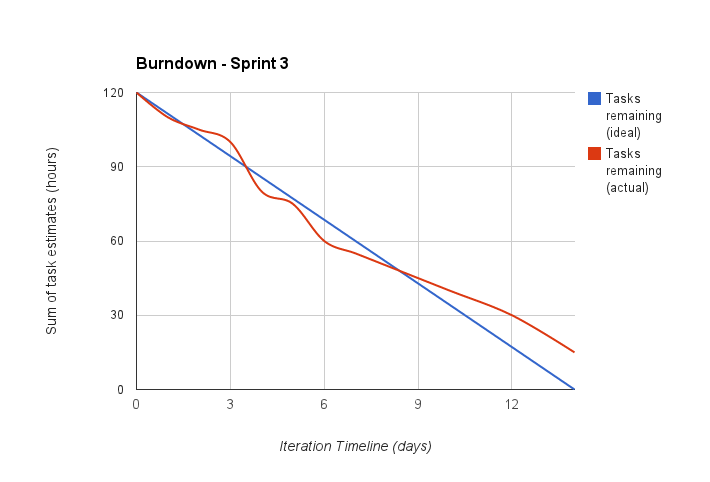
\includegraphics[scale=0.60]{../Figures/burndownSprint3.png}
\caption{Burndown chart Sprint 3}
\label{figure:burndownsprint3}
\end{figure}

\section{Evaluation}

All in all this sprint was successful.
However, refactoring was an unexpectedly time-consuming task.
Luckly, since all refactoring had been performed on a separte branch on Git, it didn't hinder
or delay any other activity as we always had a working branch for development and demonstration purposes.


